\section{Invasive Species Trade-Off Model Discussion}

\subsection{Model Generalization}

When applying our model to a larger sample of foreign plants to classify them as invasive or not invasive, it would be immensely beneficial to create an auto-classification system. Such a classification system would consist of a "line of division" in a plot where each axis would represent the ecological or economic scores. Since we do not have enough data points to create such a classification system, we propose a \textit{DSD} framework (Data-Score-Divide) below in which an environmental scientist may use our trade-off model.

In our proposed \textit{DSD} framework, environmental scientists perform the following steps as described in Figure~\ref{fig:dsdprocess}. First, a scientist must collect regional native population data, economic costs and revenues from similar firms, and collect dollar-value human risk costs in local populations. Next, data is to be evaluated via our proposed ecological and economic scores. Finally, scores for each foreign species should be plotted on an economic vs ecological score plot, where a line of division must be drawn by an evaluator to specify the split between invasive and simply foreign species. This division process is inspired by Support Vector Machines, which are commonly used in machine learning classification tasks \cite{ieeeSupportVector}.

% https://ieeexplore.ieee.org/document/708428

\begin{figure}[h!]
\centering
    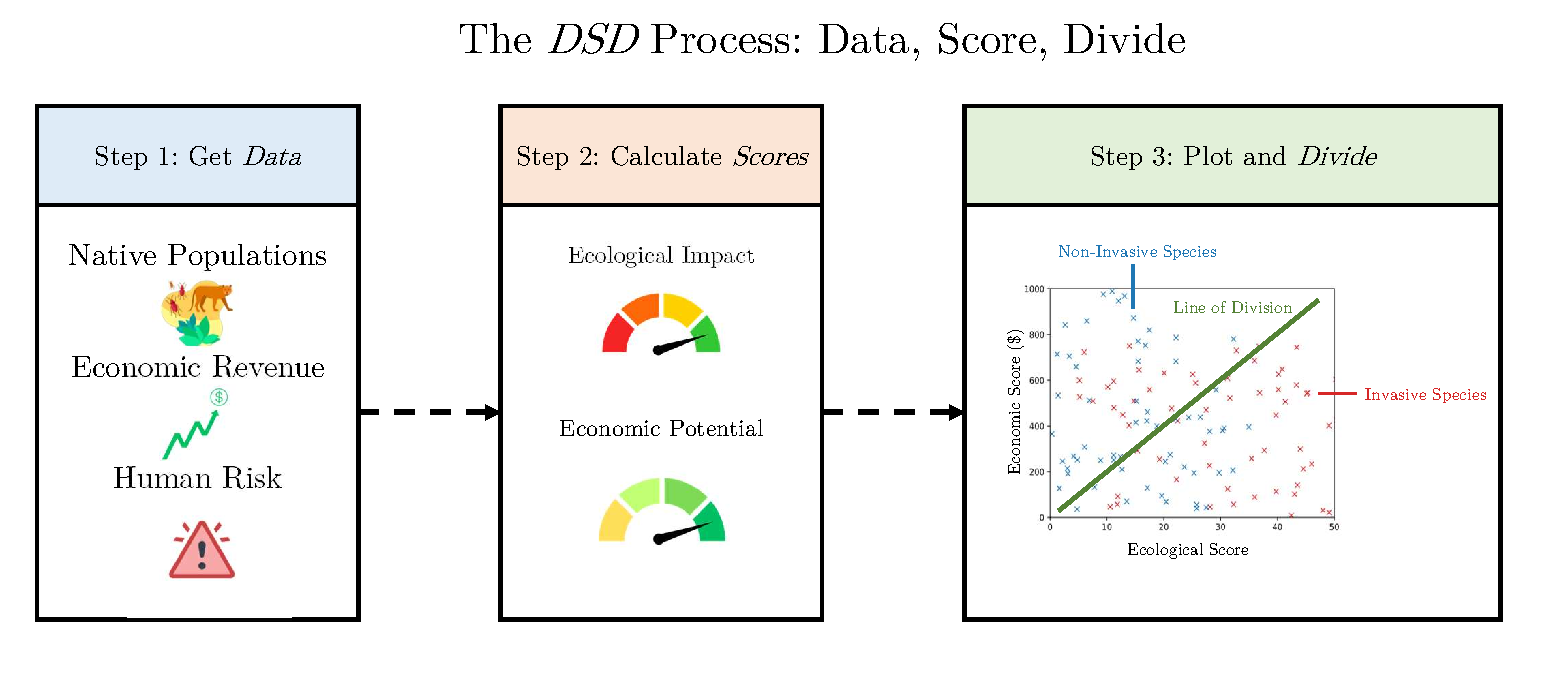
\includegraphics[scale=0.5]{figures/dsdprocess.pdf}
    \captionsetup{width=0.9\textwidth}
    \caption{\textbf{The \textit{Data-Score-Divide} (DSD) framework for evaluating invasive species.}}
    \label{fig:dsdprocess}
\end{figure}

\subsection{Strengths}
\begin{enumerate}
    \item Our model offers unique\textbf{ insights into the trade-offs} of foreign species, in particular, invasive species.
    \begin{quote}
        Unlike most foreign species impact models, which only examine the ecological benefits and downfalls of a foreign species, we examine both all trade-offs of a foreign species, both ecologically and economically.
    \end{quote}
    \item Our model is adaptable to virtually \textbf{any region and foreign plant} combination.
    \begin{quote}
        This means that our model can be applied to different scenarios and contexts, such as invasive species management, biodiversity conservation, and ecological restoration. Our model can adapt based on different regional native plants and economical conditions, and provides a general-use framework.
    \end{quote}
\end{enumerate}
\subsection{Limitations}
\begin{enumerate}
\item Intra-population dynamics between foreign and native species that are not as well known \textbf{can be difficult to predict}.
    \begin{quote}
     In the previous three contexts of analyzing the trade-offs between dandelion, garlic mustard, and English ivy plants, the most distinct aspect of these species is that they are widely classified as invasive or as a "weed." This means that they naturally tend to have a dominant nature in population dynamics, and easily outgrow native species in their habitats.
    \end{quote}
\item Economic benefits and pitfalls \textbf{may not have historical data} to take example from.
\begin{quote}
    In our analysis of dandelion and English ivy plants, several businesses that center around dandelion and English ivy harvesting already exist. This allows us to build off of previously existing work to calculate optimal economic profits and yield. However, when we take a look at the case of garlic mustard plants, few if any firms exist that center around garlic mustard harvesting, which makes one's job difficult to predict economic outcomes.
\end{quote}
    
\end{enumerate}

